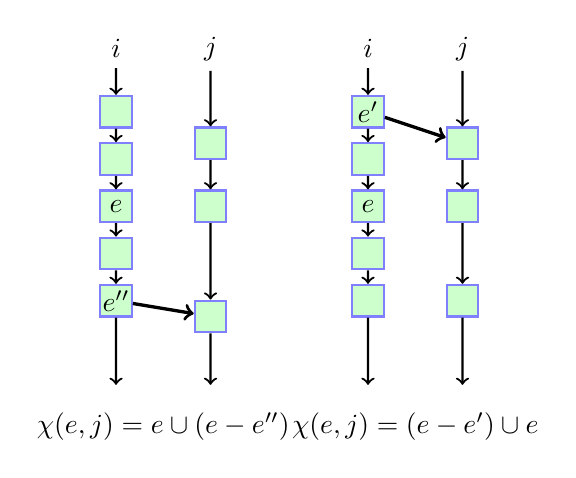
\begin{tikzpicture}[scale=0.4]

	\node 	(ge0')		at	(-8,10) 	[rectangle, thick]{$i$};

	\node 	(ge1')		at	(-8,8) 	[rectangle, thick, draw=blue!50,fill=green!20,inner sep=0pt,minimum size=.4cm]{$e'$};

	\node 	(ge5')		at	(-8,6.5) 	[rectangle, thick, draw=blue!50,fill=green!20,inner sep=0pt,minimum size=.4cm]{$$};


	\node 	(ge2')		at	(-8,5) 	[rectangle, thick, draw=blue!50,fill=green!20,inner sep=0pt,minimum size=.4cm]{$e$};

	\node 	(ge6')		at	(-8,3.5) 	[rectangle, thick, draw=blue!50,fill=green!20,inner sep=0pt,minimum size=.4cm]{$$};

	\node 	(ge3')		at	(-8,2) 	[rectangle, thick, draw=blue!50,fill=green!20,inner sep=0pt,minimum size=.4cm]{$$};

	\node 	(ge4')		at	(-8,-1) 	[rectangle, thick]{};

	\draw[->, thick]	(ge0')	to	node[auto]{}	(ge1');
	\draw[->, thick]	(ge1')	to	node[auto]{}	(ge5');
	\draw[->, thick]	(ge5')	to	node[auto]{}	(ge2');
	\draw[->, thick]	(ge2')	to	node[auto]{}	(ge6');
	\draw[->, thick]	(ge6')	to	node[auto]{}	(ge3');
	\draw[->, thick]	(ge3')	to	node[auto]{}	(ge4');

	\node 	(gf0')		at	(-5,10) 	[rectangle, thick]{$j$};

	\node 	(gf1')		at	(-5,7) 	[rectangle, thick, draw=blue!50,fill=green!20,inner sep=0pt,minimum size=.4cm]{$$};

	\node 	(gf2')		at	(-5,5) 	[rectangle, thick, draw=blue!50,fill=green!20,inner sep=0pt,minimum size=.4cm]{$$};

	\node 	(gf3')		at	(-5,2) 	[rectangle, thick, draw=blue!50,fill=green!20,inner sep=0pt,minimum size=.4cm]{$$};

	\node 	(gf4')		at	(-5,-1) 	[rectangle, thick]{};

	\draw[->, thick]	(gf0')	to	node[auto]{}	(gf1');
	\draw[->, thick]	(gf1')	to	node[auto]{}	(gf2');
	\draw[->, thick]	(gf2')	to	node[auto]{}	(gf3');
	\draw[->, thick]	(gf3')	to	node[auto]{}	(gf4');

	\draw[->, very thick]	(ge1')	to	node[auto]{}	(gf1');
%	\draw[->, very thick]	(gf2')	to	node[auto]{}	(ge2');
%	\draw[->, very thick]	(gf3')	to	node[auto]{}	(ge3');

	\node 	(g')		at	(-6.5,-2) 	[rectangle, thick]{$\chi(e,j)=(\down e -\down e')\cup \up e$};
%----------------------------------------------------------------------------------------------


	\node 	(ge0)		at	(-16,10) 	[rectangle, thick]{$i$};

	\node 	(ge1)		at	(-16,8) 	[rectangle, thick, draw=blue!50,fill=green!20,inner sep=0pt,minimum size=.4cm]{$$};

	\node 	(ge5)		at	(-16,6.5) 	[rectangle, thick, draw=blue!50,fill=green!20,inner sep=0pt,minimum size=.4cm]{$$};


	\node 	(ge2)		at	(-16,5) 	[rectangle, thick, draw=blue!50,fill=green!20,inner sep=0pt,minimum size=.4cm]{$e$};

	\node 	(ge6)		at	(-16,3.5) 	[rectangle, thick, draw=blue!50,fill=green!20,inner sep=0pt,minimum size=.4cm]{$$};


	\node 	(ge3)		at	(-16,2) 	[rectangle, thick, draw=blue!50,fill=green!20,inner sep=0pt,minimum size=.4cm]{$e''$};

	\node 	(ge4)		at	(-16,-1) 	[rectangle, thick]{};

	\draw[->, thick]	(ge0)	to	node[auto]{}	(ge1);
	\draw[->, thick]	(ge1)	to	node[auto]{}	(ge5);
	\draw[->, thick]	(ge5)	to	node[auto]{}	(ge2);
	\draw[->, thick]	(ge2)	to	node[auto]{}	(ge6);
	\draw[->, thick]	(ge6)	to	node[auto]{}	(ge3);
	\draw[->, thick]	(ge3)	to	node[auto]{}	(ge4);

	\node 	(gf0)		at	(-13,10) 	[rectangle, thick]{$j$};

	\node 	(gf1)		at	(-13,7) 	[rectangle, thick, draw=blue!50,fill=green!20,inner sep=0pt,minimum size=.4cm]{$$};

	\node 	(gf2)		at	(-13,5) 	[rectangle, thick, draw=blue!50,fill=green!20,inner sep=0pt,minimum size=.4cm]{$$};

	\node 	(gf3)		at	(-13,1.5) 	[rectangle, thick, draw=blue!50,fill=green!20,inner sep=0pt,minimum size=.4cm]{$$};

	\node 	(gf4)		at	(-13,-1) 	[rectangle, thick]{};

	\draw[->, thick]	(gf0)	to	node[auto]{}	(gf1);
	\draw[->, thick]	(gf1)	to	node[auto]{}	(gf2);
	\draw[->, thick]	(gf2)	to	node[auto]{}	(gf3);
	\draw[->, thick]	(gf3)	to	node[auto]{}	(gf4);

%	\draw[->, very thick]	(gf1)	to	node[auto]{}	(ge2);
%	\draw[->, very thick]	(gf2)	to	node[auto]{}	(ge2);
	\draw[->, very thick]	(ge3)	to	node[auto]{}	(gf3);

	\node 	(g)		at	(-14.5,-2) 	[rectangle, thick]{$\chi(e,j)=\down e \cup (\up e -\up e'')$};
%
\end{tikzpicture}

